\documentclass[12pt, a4paper]{article}
\usepackage[lmargin =0.5 in, 
rmargin=0.5in, 
tmargin=1in,
bmargin=0.5in]{geometry}
\geometry{letterpaper}
\usepackage{tikz-cd}
\usepackage{amsmath}
\usepackage{amssymb}
\usepackage{blindtext}
\usepackage{titlesec}
\usepackage{enumitem}
\usepackage{fancyhdr}
\usepackage{amsthm}
\usepackage{graphicx}
\usepackage{cool}
\usepackage{thmtools}
\usepackage{hyperref}
\graphicspath{ }					%path to an image

%-------- sexy font ------------%
%\usepackage{libertine}
%\usepackage{libertinust1math}

%\usepackage{mlmodern}				% very nice and classic
%\usepackage[utopia]{mathdesign}
%\usepackage[T1]{fontenc}


\usepackage{mlmodern}
\usepackage{eulervm}
%\usepackage{tgtermes} 				%times new roman
%-------- sexy font ------------%


% Problem Styles
%====================================================================%


\newtheorem{problem}{Problem}


\theoremstyle{definition}
\newtheorem{thm}{Theorem}
\newtheorem{lemma}{Lemma}
\newtheorem{prop}{Proposition}
\newtheorem{cor}{Corollary}
\newtheorem{fact}{Fact}
\newtheorem{defn}{Definition}
\newtheorem{example}{Example}
\newtheorem{question}{Question}

\newtheorem{manualprobleminner}{Problem}

\newenvironment{manualproblem}[1]{%
	\renewcommand\themanualprobleminner{#1}%
	\manualprobleminner
}{\endmanualprobleminner}

\newcommand{\penum}{ \begin{enumerate}[label=\bf(\alph*), leftmargin=0pt]}
	\newcommand{\epenum}{ \end{enumerate} }

% Math fonts shortcuts
%====================================================================%

\newcommand{\ring}{\mathcal{R}}
\newcommand{\N}{\mathbb{N}}                           % Natural numbers
\newcommand{\Z}{\mathbb{Z}}                           % Integers
\newcommand{\R}{\mathbb{R}}                           % Real numbers
\newcommand{\C}{\mathbb{C}}                           % Complex numbers
\newcommand{\F}{\mathbb{F}}                           % Arbitrary field
\newcommand{\Q}{\mathbb{Q}}                           % Arbitrary field
\newcommand{\PP}{\mathcal{P}}                         % Partition
\newcommand{\M}{\mathcal{M}}                         % Mathcal M
\newcommand{\eL}{\mathcal{L}}                         % Mathcal L
\newcommand{\T}{\mathbb{T}}                         % Mathcal T
\newcommand{\U}{\mathcal{U}}                         % Mathcal U\\
\newcommand{\V}{\mathcal{V}}                         % Mathcal V

% symbol shortcuts
%====================================================================%

\newcommand{\bd}{\partial}
\newcommand{\grad}{\nabla}
\newcommand{\lam}{\lambda}
\newcommand{\imp}{\implies}
\newcommand{\all}{\forall}
\newcommand{\exs}{\exists}
\newcommand{\delt}{\delta}
\newcommand{\ep}{\varepsilon}
\newcommand{\ra}{\rightarrow}
\newcommand{\vph}{\varphi}

\newcommand{\ol}{\overline}
\newcommand{\f}{\frac}
\newcommand{\lf}{\lfrac}
\newcommand{\df}{\dfrac}

% bracketting shortcuts
%====================================================================%
\newcommand{\abs}[1]{\left| #1 \right|}
\newcommand{\babs}[1]{\Big|#1\Big|}
\newcommand{\bound}{\Big|}
\newcommand{\BB}[1]{\left(#1\right)}
\newcommand{\dd}{\mathrm{d}}
\newcommand{\artanh}{\mathrm{artanh}}
\newcommand{\Med}{\mathrm{Med}}
\newcommand{\Cov}{\mathrm{Cov}}
\newcommand{\Corr}{\mathrm{Corr}}
\newcommand{\tr}{\mathrm{tr}}
\newcommand{\Range}[1]{\mathrm{range}(#1)}
\newcommand{\Null}[1]{\mathrm{null}(#1)}
\newcommand{\lan}{\langle}
\newcommand{\ran}{\rangle}
\newcommand{\norm}[1]{\left\lVert#1\right\rVert}
\newcommand{\inn}[1]{\lan#1\ran}
\newcommand{\op}[1]{\operatorname{#1}}
\newcommand{\bmat}[1]{\begin{bmatrix}#1\end{bmatrix}}
\newcommand{\pmat}[1]{\begin{pmatrix}#1\end{pmatrix}}
\newcommand{\vmat}[1]{\begin{vmatrix}#1\end{vmatrix}}

\newcommand{\amogus}{{\bigcap}\kern-0.8em\raisebox{0.3ex}{$\subset$}}
\newcommand{\Note}{\textbf{Note: }}
\newcommand{\Aside}{{\bf Aside: }}
%restriction
%\newcommand{\op}[1]{\operatorname{#1}}
%\newcommand{\done}{$$\mathcal{QED}$$}

%====================================================================%


\setlength{\parindent}{0pt}      	% No paragraph indentations
\pagestyle{fancy}
\fancyhf{}							% fancy header

\setcounter{secnumdepth}{0}			% sections are numbered but numbers do not appear
\setcounter{tocdepth}{2} 			% no subsubsections in toc

%template
%====================================================================%
%\begin{manualproblem}{1}
%Spivak.
%\end{manualproblem}

%\begin{proof}[Solution]
%\end{proof}

%----------- or -----------%

%\begin{problem} 		
%\end{problem}	

%\penum
%	\item
%\epenum
%====================================================================%


\newcommand{\Course}{351}
\newcommand{\hwNumber}{3}

%preamble

\title{}
\author{A.N.}
\date{\today}
\lhead{\Course A\hwNumber}
\rhead{\thepage}
%\cfoot{\thepage}


%====================================================================%
\begin{document}



\begin{problem}
\end{problem}
We determine a formula for the solution to the following IVP using the method of characteristics:
$$\begin{cases} 
	u_t + V \cdot \nabla u = -cv + f(x,t) \\
	u(x,0) = g(x).
\end{cases}$$
Let $\vec{x}(s) ,t(s)  $ be a characteristic curve parametrized by $s$, and define $z(s) = u(\vec{x}(s), t(s))$ so that $$\dot{z}(s) = u_t \dot{t} +\dot{ \vec{x}} \cdot \nabla u = -cz + f(\vec{x}(s), t(s)).$$
By the PDE we aim to solve the new IVP 
$$
\begin{cases}
	\dot{t} = 1 & t(0) = 0\\
	\dot{\vec{x}} = v & \vec{x}(0) = v_0\\
	\dot{z} = -cz + f & z(0) = g(v_0). 
\end{cases}$$
We can see that $t(s) = s, x = sv + v_0$, and by Duhamels Principle, we can compute
$$z(s) = Ae^{-cs}  + \int_0^s e^{-c(s-k)}f(x(k), t(k)) dk.$$ 
Since $z(0)= g(v_0)$, we must have that $A = g(v_0)$. Writing $t=s, v_0 = x-tv$, we find that 
$$u(x,t) = g(x-tv) + \int_{0}^t e^{-c(t-k)} f((k-t)v + x, k) dk. $$
 \newpage 
\begin{problem}
\end{problem}
Let $\phi(x) = u(x,0)$. From our disussion in class the charcteristic equations of the PDE take the form of $(x_0 + \phi(x_0)s,s)$ for $s>0$. 
Since $\phi(x)$ vanishes outside of $(-1,-1)$, the characteristic curves will just be vertical lines. For $x_0\in (-1,1)$, we can write $t = \frac{1}{\phi(x_0)} x - \frac{x_0}{\phi(x_0)}$. The corresponding characteristic curves will look as follows:
$$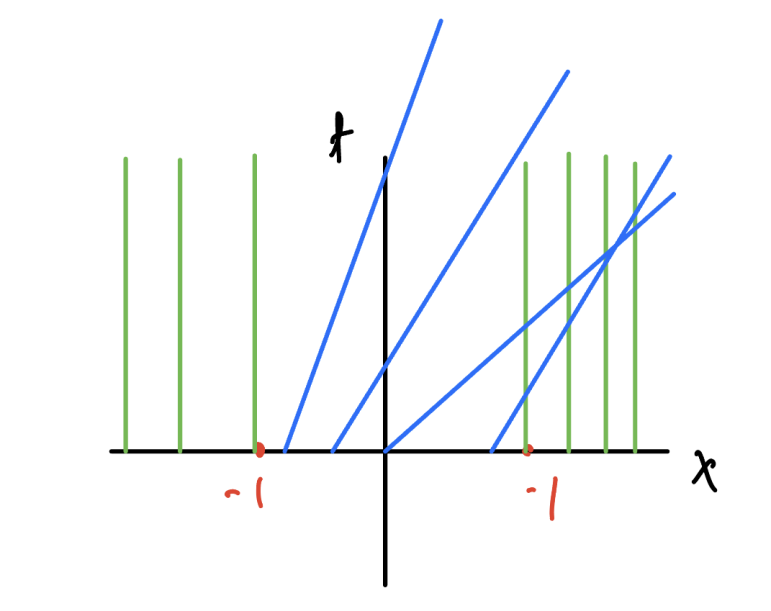
\includegraphics[scale = 0.3]{mat351A3Q2}$$
We now determine the first time $t$ where the characteristic lines will intersect. First consider when two non vertical lines intercept one another. Note that two lines will intercept when the following holds: 
$$\frac{1}{\phi(a)} x - \frac{a}{\phi(a)} = \frac{1}{\phi(b)} x - \frac{b}{\phi(b)} \iff x = \frac{a\phi(b) - b\phi(a)}{\phi(b) - \phi(a)}.$$
There will be 3 distinct cases corresonding to $0\leq a,b<1, -1<a<0<b<1, -1<a,b<0$, where we can write $\phi$ as: 
$$\begin{cases}
	\phi(a) = 1-a, \phi(b) = 1-b\\
	\phi(a) = 1+a, \phi(b) = 1-b\\
	\phi(a) = 1+a, \phi(b) = 1+b
\end{cases}$$
In the first case we solve and see that $x=1$ and so $t=1$ for that family of lines. 
In the second case we get that $x = 1 - \frac{2ab}{a-b}$, which will result in the values attained at $x$ to be greater than $1$ along those lines. In the third case we have that $x= -1$, which the lines are not defined at. Since all the lines are increasing, the minimum intersection will occur at most at the first of the vertical family of lines. Therefore the first time that the intersect will be at $t=1$. 
We finally solve the PDE. Let $x(s), t(s)$ be characteristic curves of the PDE. Let $z(s) = u(x(s), t(s))$, by the PDE we have: 
$$\begin{cases} 
	\dot{t} = 1 &t(0) = 0\\
	\dot{x} =z & x(0) = x_0\\
	\dot{z} = 0 & z(0) = \max{(1-|x_0|,0) }
\end{cases}$$
We solve this as 
$$\begin{cases}
t = s\\
	x = x_0 + \phi(x_0)t\\
	z = \phi(x_0)
\end{cases}$$
For $x_0>0$, we can write $$x = x_0 +t  \frac{1 - x_0 +|-1+x_0|}{2}.$$
Solving using the quadratic formula we get $$x_0 = \frac{x-t}{1-t}, t\neq1.$$
Similarly we solve this as $x_0 = \frac{x-t}{t+1} , t\neq 1$. Thus we can write $$u(x,t) =z = \phi(x_0) = \max\left( 1 - \left| \frac{x-t}{t-1} \right|, 0 \right)$$ in the region where $0<t<1$. For $x_0<0$ we get another solution 
given by $$x_0 = \frac{x-t}{t+1},$$ so $$u(x,t) = \max\left( 1 - \left|\frac{x-t}{t+1} \right|,0 \right).$$
 \newpage 
\begin{problem}
\end{problem}
We compute the discriminant of the PDE $(1+x)u_{xx} + 2xyu_{xy} - y^2u_{yy} =0$  as follows:
$$D= (xy)^2 - (1+x\cdot -y^2)= y^2(x^2+x+1).$$
First note that this PDE is never elliptic since $y^2\geq 0$ and $x^2+x+1>0$ for all $x,y$.
This PDE will be parabolic exactly when $y=0$, since $x^2+x+1 >0$. 
Finally it will be hyperbolic everywhere else i.e. $y\neq 0, x\in \R$. 
 \newpage 
\begin{problem}
\end{problem}
We make the change of variables $\xi = x, \eta = 2x+y$. This gives us that $\partial_\eta = \partial_y, \partial_\xi = \partial_x + 2\partial_y$.This reduces the PDE to the form $u_{\xi \xi} = 0$.
We get that $u_\xi = f(\eta)$, and so $u = \xi f(\eta) + g(\eta)$ i.e. $u = xf(2x+y) + g(2x+y)$. 
We now solve for the particular solution. We first solve the following PDE: 
$$(\partial_x - 2\partial_y ) v = e^{2x+y}.$$ Let $(x(s),y(s))$ be a characteristic curve. Let $z(s) = v(x(s), y(s))$, so that the following system of ODE's holds: 
$$\begin{cases}
	\dot(x) = 1 & x(0) = c\\
	\dot{y} = -2 & y(0) = d\\
	\dot{z} = e^{2x(s) + y(s)} & z(0) = 1
\end{cases}$$
We solve this as $x =s+c, y = -2s+d$, and so $\dot{z}(s) = e^{2c+d}$, thus $z(s) = se^{2c+d} = xe^{2x+y}$ if we choose our initial condition $c=0$. We now do this again to the PDE $$(\partial_x - 2\partial_y) u = xe^{2x+y}. $$
We let $x(s), y(s)$ be a characteristic curve of the PDE, and let $z(s) = u(x(s),y(s))$ so that $$\dot{z}(s) = x(s) e^{2x(s) + y(s)} = u_x \dot{x} + u_y \dot{y}.$$
We have by the PDE that $\dot{x} = 1, \dot{y} = -2$. So $x = s+ c, y = -2s+d$. Therefore we have that $$\dot{z} (s) = (s+c) e^{2c+d} \implies z(s) = \frac{1}{2} s^2 e^{2c+d} + cs e^{2c+d}. $$
We can choose initial condition $c=0$, to get the solution as $u(x,y) = \frac{1}{2}x^2 e^{2x+y}$. 
Therefore a general solution to this PDE will be of the form: 
$$u(x,y) = xf(2x+y) + g(2x+y) + \frac{1}{2} x^2 e^{2x+y}. $$
 \newpage 
\begin{problem}
\end{problem}
By D'Almberts Formula, the solution to the PDE with the given initial values is: 
$$u(x,y) = \frac{1}{2c} \int_{x-tc} \mathbbm{1}_{(-a,a)}dy$$
For $t = k \frac{a}{2c}$, $k = 0,1,2,3,4,5$, we have the following snapshots of the behaviour of $u:$. 
$$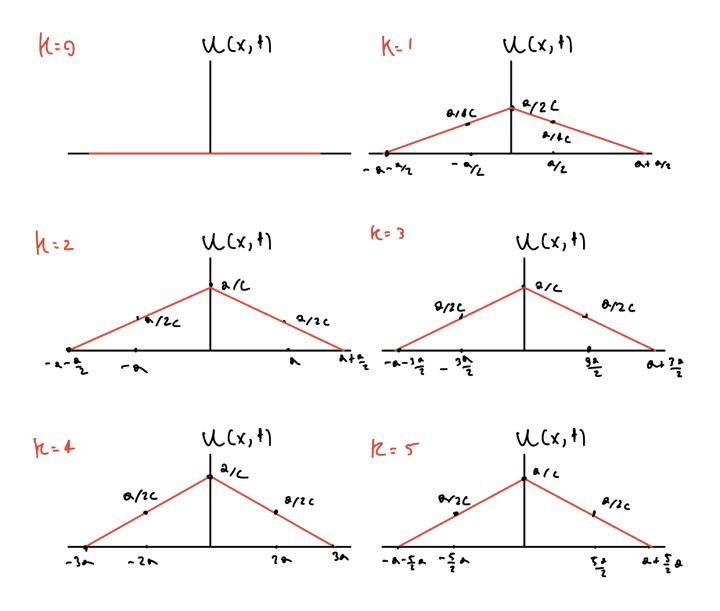
\includegraphics[width = \textwidth]{mat351A3Q5}$$
We note that this obeys the finite speed condition. 
\end{document}
